\documentclass[12pt,a4paper]{article}

\usepackage[utf8]{inputenc}
\usepackage[spanish]{babel}
\usepackage[margin=2.5cm]{geometry}
\usepackage{graphicx}
\usepackage{booktabs}
\usepackage{longtable}
\usepackage{array}
\usepackage{enumitem}
\usepackage{listings}
\usepackage{xcolor}
\usepackage{fancyhdr}
\usepackage{caption}

\definecolor{sqlkeyword}{rgb}{0.0, 0.0, 0.7}
\definecolor{sqlcomment}{rgb}{0.4, 0.4, 0.4}
\definecolor{sqlstring}{rgb}{0.0, 0.5, 0.0}
\definecolor{codebg}{rgb}{0.96, 0.96, 0.96}

\lstdefinestyle{sql}{
    language=SQL,
    basicstyle=\ttfamily\footnotesize,
    keywordstyle=\color{sqlkeyword}\bfseries,
    commentstyle=\color{sqlcomment}\itshape,
    stringstyle=\color{sqlstring},
    backgroundcolor=\color{codebg},
    frame=single,
    breaklines=true,
    showstringspaces=false,
    tabsize=2,
    morekeywords={ENUM,IDENTITY,RETURNING,INOUT,IMMUTABLE,CALL,
                  DECIMAL,BOOLEAN,SERIAL,CASCADE,RESTRICT,GENERATED,
                  ALWAYS,COALESCE,NULLIF,FILTER,PARTITION},
    literate={á}{{\'a}}1 {é}{{\'e}}1 {í}{{\'i}}1 {ó}{{\'o}}1 {ú}{{\'u}}1
             {ñ}{{\~n}}1 {Á}{{\'A}}1 {É}{{\'E}}1 {Í}{{\'I}}1 {Ó}{{\'O}}1
             {Ú}{{\'U}}1 {Ñ}{{\~N}}1,
}
\lstset{style=sql}

\pagestyle{fancy}
\fancyhf{}
\fancyhead[L]{\small Playoff Hoops --- DER, Tablas y Vistas}
\fancyhead[R]{\small CMP 4002}
\fancyfoot[C]{\thepage}

\title{\textbf{Playoff Hoops}\\[0.3cm]
{\large Diagrama Entidad-Relaci\'on, Tablas y Vistas}}
\author{Juli\'an Le\'on}
\date{Abril 2026}

\begin{document}
\maketitle

% =============================================================
% 1. DER
% =============================================================
\section{Diagrama Entidad-Relaci\'on}

El esquema est\'a en FNBC con 13 tablas (10 entidades + 3 junciones M:M con atributos).
Todas las relaciones muchos-a-muchos se resuelven mediante tablas de junci\'on con atributos
significativos (no diccionarios).

\begin{figure}[h!]
    \centering
    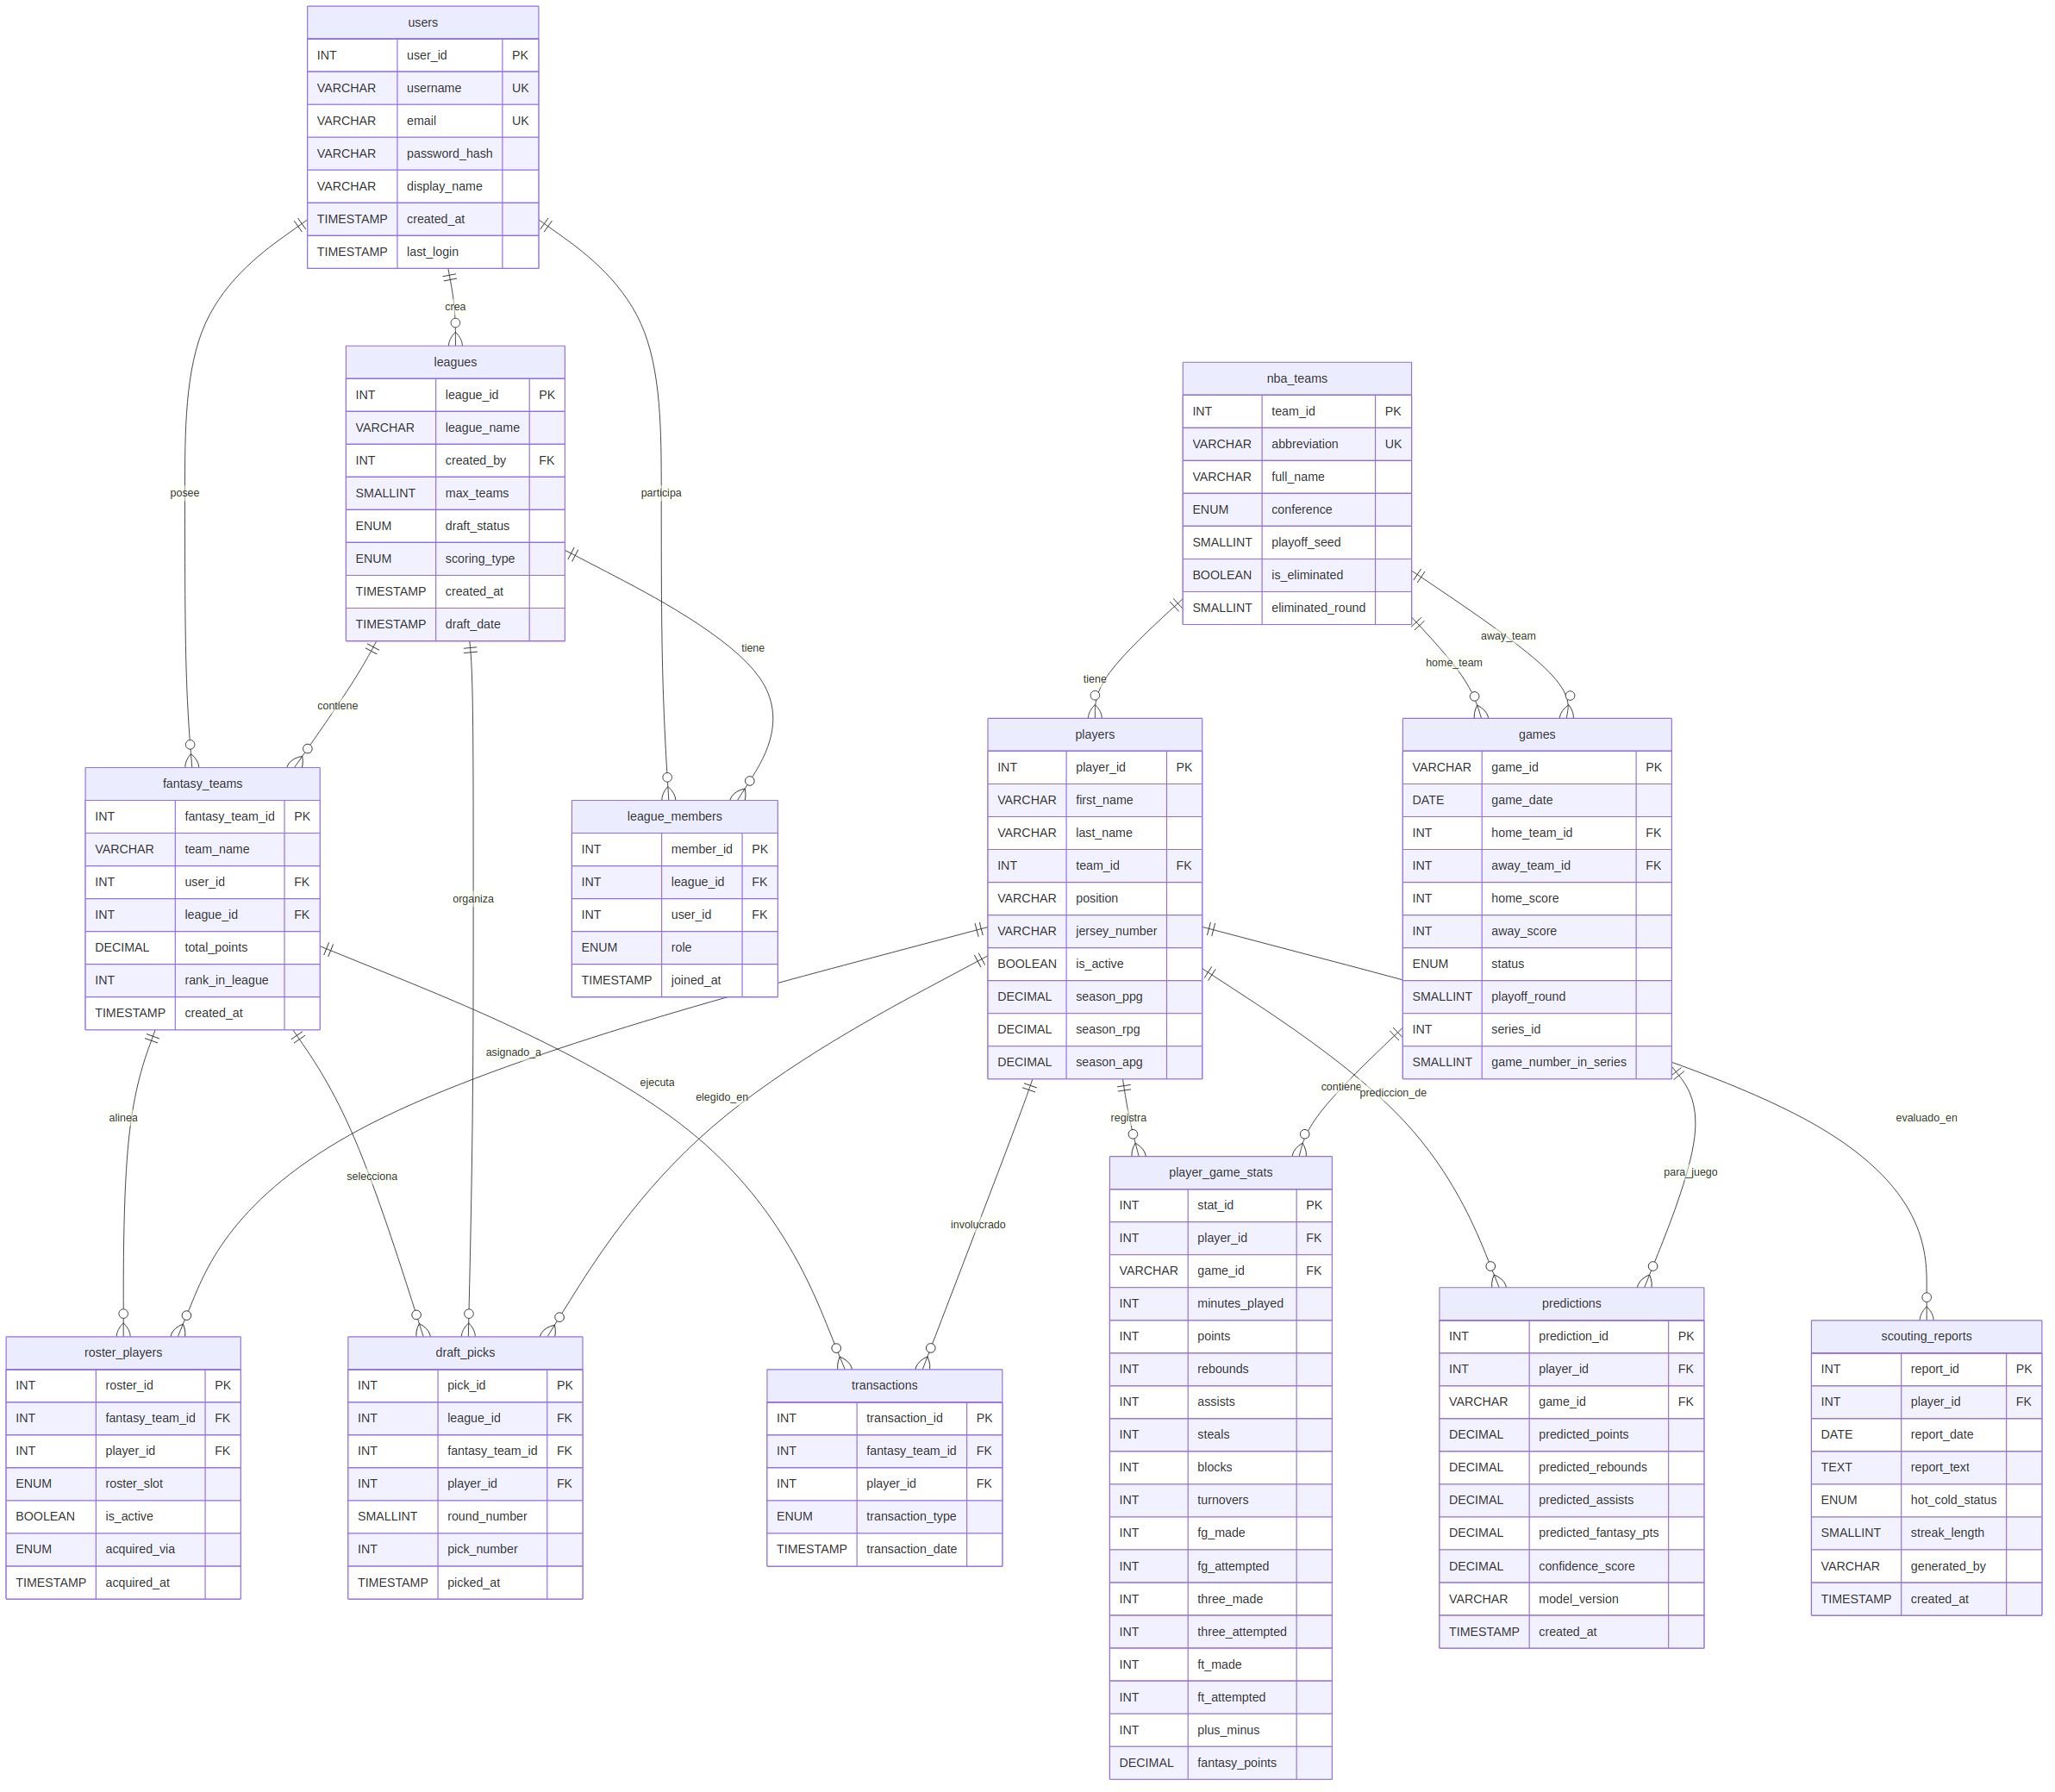
\includegraphics[width=\textwidth]{DER.png}
    \caption{DER --- Playoff Hoops (13 tablas, 20 relaciones FK)}
    \label{fig:der}
\end{figure}

% =============================================================
% 2. CARDINALIDADES
% =============================================================
\section{Cardinalidades}

\begin{longtable}{p{6cm} c p{6.5cm}}
\toprule
\textbf{Relaci\'on} & \textbf{Card.} & \textbf{Descripci\'on} \\
\midrule
\endhead
nba\_teams $\to$ players & 1:N & Un equipo tiene muchos jugadores \\
nba\_teams $\to$ games (home) & 1:N & Un equipo juega muchos partidos como local \\
nba\_teams $\to$ games (away) & 1:N & Un equipo juega muchos partidos como visitante \\
players $\leftrightarrow$ games & M:N & V\'ia \texttt{player\_game\_stats} (15 attrs) \\
users $\to$ leagues (created\_by) & 1:N & Un usuario crea muchas ligas \\
users $\leftrightarrow$ leagues & M:N & V\'ia \texttt{league\_members} (role, joined\_at) \\
users $\to$ fantasy\_teams & 1:N & Un usuario posee equipos fantasy \\
leagues $\to$ fantasy\_teams & 1:N & Una liga contiene equipos \\
fantasy\_teams $\leftrightarrow$ players & M:N & V\'ia \texttt{roster\_players} (slot, via, active) \\
leagues $\to$ draft\_picks & 1:N & Una liga tiene picks de draft \\
fantasy\_teams $\to$ draft\_picks & 1:N & Un equipo hace picks \\
fantasy\_teams $\to$ transactions & 1:N & Un equipo ejecuta transacciones \\
players $\to$ predictions & 1:N & Un jugador tiene predicciones \\
games $\to$ predictions & 1:N & Un juego tiene predicciones \\
players $\to$ scouting\_reports & 1:N & Un jugador tiene reportes \\
\bottomrule
\end{longtable}

% =============================================================
% 3. TABLAS DE ENTIDAD
% =============================================================
\section{Tablas de Entidad (10)}

\subsection{\texttt{users} --- Usuarios del sistema}
\begin{tabular}{>{\ttfamily\small}l l l p{5.5cm}}
\toprule
\normalfont\textbf{Columna} & \textbf{Tipo} & \textbf{Constraint} & \textbf{Descripci\'on} \\
\midrule
user\_id & INT & PK (IDENTITY) & Identificador \'unico autogenerado \\
username & VARCHAR(50) & UNIQUE, NOT NULL & Nombre de usuario \\
email & VARCHAR(100) & UNIQUE, NOT NULL & Correo electr\'onico \\
password\_hash & VARCHAR(255) & NOT NULL & Hash bcrypt de la contrase\~na \\
display\_name & VARCHAR(100) & & Nombre para mostrar \\
created\_at & TIMESTAMP & NOT NULL, DEFAULT NOW() & Fecha de registro \\
last\_login & TIMESTAMP & & \'Ultimo acceso \\
\bottomrule
\end{tabular}

\subsection{\texttt{nba\_teams} --- Equipos NBA reales}
\begin{tabular}{>{\ttfamily\small}l l l p{5cm}}
\toprule
\normalfont\textbf{Columna} & \textbf{Tipo} & \textbf{Constraint} & \textbf{Descripci\'on} \\
\midrule
team\_id & INT & PK & ID oficial de la NBA \\
abbreviation & VARCHAR(3) & UNIQUE, NOT NULL & Ej: LAL, BOS, OKC \\
full\_name & VARCHAR(100) & NOT NULL & Nombre completo del equipo \\
conference & ENUM & NOT NULL & East / West \\
playoff\_seed & SMALLINT & CHECK 1--16 & Semilla en playoffs \\
is\_eliminated & BOOLEAN & NOT NULL, DEFAULT FALSE & Eliminado del playoff \\
eliminated\_round & SMALLINT & CHECK 1--4 & Ronda de eliminaci\'on \\
\bottomrule
\end{tabular}

\subsection{\texttt{players} --- Jugadores NBA}
\begin{tabular}{>{\ttfamily\small}l l l p{5cm}}
\toprule
\normalfont\textbf{Columna} & \textbf{Tipo} & \textbf{Constraint} & \textbf{Descripci\'on} \\
\midrule
player\_id & INT & PK & ID oficial de la NBA \\
first\_name & VARCHAR(50) & NOT NULL & Nombre \\
last\_name & VARCHAR(50) & NOT NULL & Apellido \\
team\_id & INT & FK $\to$ nba\_teams, NOT NULL & Equipo actual \\
position & VARCHAR(5) & NOT NULL & G, F, C, G-F, F-C \\
jersey\_number & VARCHAR(3) & & N\'umero de camiseta \\
is\_active & BOOLEAN & NOT NULL, DEFAULT TRUE & Activo en la liga \\
season\_ppg & DECIMAL(5,2) & DEFAULT 0 & Promedio puntos/partido \\
season\_rpg & DECIMAL(5,2) & DEFAULT 0 & Promedio rebotes/partido \\
season\_apg & DECIMAL(5,2) & DEFAULT 0 & Promedio asistencias/partido \\
\bottomrule
\end{tabular}

\subsection{\texttt{games} --- Partidos NBA}
\begin{tabular}{>{\ttfamily\small}l l l p{4.5cm}}
\toprule
\normalfont\textbf{Columna} & \textbf{Tipo} & \textbf{Constraint} & \textbf{Descripci\'on} \\
\midrule
game\_id & VARCHAR(20) & PK & ID oficial de la NBA \\
game\_date & DATE & NOT NULL & Fecha del partido \\
home\_team\_id & INT & FK $\to$ nba\_teams, NOT NULL & Equipo local \\
away\_team\_id & INT & FK $\to$ nba\_teams, NOT NULL & Equipo visitante \\
home\_score & INT & DEFAULT 0 & Puntos local \\
away\_score & INT & DEFAULT 0 & Puntos visitante \\
status & ENUM & NOT NULL, DEFAULT scheduled & scheduled/live/final \\
playoff\_round & SMALLINT & NOT NULL, CHECK 1--4 & 1=R1, 2=Semis, 3=CF, 4=Finals \\
series\_id & INT & & Identificador de la serie \\
game\_number\_in\_series & SMALLINT & & Juego \# en la serie \\
\bottomrule
\end{tabular}

\textbf{CHECK:} \texttt{home\_team\_id <> away\_team\_id} (un equipo no juega contra s\'i mismo).

\subsection{\texttt{leagues} --- Ligas fantasy}
\begin{tabular}{>{\ttfamily\small}l l l p{5cm}}
\toprule
\normalfont\textbf{Columna} & \textbf{Tipo} & \textbf{Constraint} & \textbf{Descripci\'on} \\
\midrule
league\_id & INT & PK (IDENTITY) & Identificador \'unico \\
league\_name & VARCHAR(100) & NOT NULL & Nombre de la liga \\
created\_by & INT & FK $\to$ users, NOT NULL & Usuario creador \\
max\_teams & SMALLINT & CHECK 2--10, DEFAULT 8 & M\'aximo de equipos \\
draft\_status & ENUM & DEFAULT pending & pending/in\_progress/completed \\
scoring\_type & ENUM & DEFAULT points & points / categories \\
created\_at & TIMESTAMP & DEFAULT NOW() & Fecha de creaci\'on \\
draft\_date & TIMESTAMP & & Fecha del draft \\
\bottomrule
\end{tabular}

\subsection{\texttt{fantasy\_teams} --- Equipos fantasy}
\begin{tabular}{>{\ttfamily\small}l l l p{4.5cm}}
\toprule
\normalfont\textbf{Columna} & \textbf{Tipo} & \textbf{Constraint} & \textbf{Descripci\'on} \\
\midrule
fantasy\_team\_id & INT & PK (IDENTITY) & Identificador \'unico \\
team\_name & VARCHAR(100) & NOT NULL & Nombre del equipo \\
user\_id & INT & FK $\to$ users, NOT NULL & Due\~no \\
league\_id & INT & FK $\to$ leagues, NOT NULL & Liga a la que pertenece \\
total\_points & DECIMAL(10,2) & DEFAULT 0 & Mantenido por trigger \\
rank\_in\_league & INT & & Posici\'on en la liga \\
created\_at & TIMESTAMP & DEFAULT NOW() & Fecha de creaci\'on \\
\bottomrule
\end{tabular}

\textbf{UNIQUE:} \texttt{(user\_id, league\_id)} --- un usuario solo puede tener un equipo por liga.

\subsection{\texttt{draft\_picks} --- Historial de draft}
\begin{tabular}{>{\ttfamily\small}l l l p{4.5cm}}
\toprule
\normalfont\textbf{Columna} & \textbf{Tipo} & \textbf{Constraint} & \textbf{Descripci\'on} \\
\midrule
pick\_id & INT & PK (IDENTITY) & Identificador \'unico \\
league\_id & INT & FK $\to$ leagues, NOT NULL & Liga del draft \\
fantasy\_team\_id & INT & FK $\to$ fantasy\_teams, NOT NULL & Equipo que selecciona \\
player\_id & INT & FK $\to$ players, NOT NULL & Jugador seleccionado \\
round\_number & SMALLINT & NOT NULL & Ronda del draft \\
pick\_number & INT & NOT NULL & N\'umero de pick global \\
picked\_at & TIMESTAMP & DEFAULT NOW() & Momento de la selecci\'on \\
\bottomrule
\end{tabular}

\textbf{UNIQUE:} \texttt{(league\_id, player\_id)} y \texttt{(league\_id, pick\_number)}.

\subsection{\texttt{transactions} --- Log de movimientos}
\begin{tabular}{>{\ttfamily\small}l l l p{5cm}}
\toprule
\normalfont\textbf{Columna} & \textbf{Tipo} & \textbf{Constraint} & \textbf{Descripci\'on} \\
\midrule
transaction\_id & INT & PK (IDENTITY) & Identificador \'unico \\
fantasy\_team\_id & INT & FK $\to$ fantasy\_teams & Equipo involucrado \\
player\_id & INT & FK $\to$ players & Jugador involucrado \\
transaction\_type & ENUM & NOT NULL & add / drop / trade \\
transaction\_date & TIMESTAMP & DEFAULT NOW() & Fecha del movimiento \\
\bottomrule
\end{tabular}

\subsection{\texttt{predictions} --- Predicciones ML}
\begin{tabular}{>{\ttfamily\small}l l l p{4.5cm}}
\toprule
\normalfont\textbf{Columna} & \textbf{Tipo} & \textbf{Constraint} & \textbf{Descripci\'on} \\
\midrule
prediction\_id & INT & PK (IDENTITY) & Identificador \'unico \\
player\_id & INT & FK $\to$ players & Jugador predicho \\
game\_id & VARCHAR(20) & FK $\to$ games & Partido objetivo \\
predicted\_points & DECIMAL(6,2) & & Puntos predichos \\
predicted\_rebounds & DECIMAL(5,2) & & Rebotes predichos \\
predicted\_assists & DECIMAL(5,2) & & Asistencias predichas \\
predicted\_fantasy\_pts & DECIMAL(7,2) & & Fantasy points predichos \\
confidence\_score & DECIMAL(4,3) & & Score de confianza (0--1) \\
model\_version & VARCHAR(20) & NOT NULL & Versi\'on del modelo \\
created\_at & TIMESTAMP & DEFAULT NOW() & Fecha de generaci\'on \\
\bottomrule
\end{tabular}

\textbf{UNIQUE:} \texttt{(player\_id, game\_id, model\_version)}.

\subsection{\texttt{scouting\_reports} --- Reportes de IA}
\begin{tabular}{>{\ttfamily\small}l l l p{4.5cm}}
\toprule
\normalfont\textbf{Columna} & \textbf{Tipo} & \textbf{Constraint} & \textbf{Descripci\'on} \\
\midrule
report\_id & INT & PK (IDENTITY) & Identificador \'unico \\
player\_id & INT & FK $\to$ players & Jugador evaluado \\
report\_date & DATE & NOT NULL & Fecha del reporte \\
report\_text & TEXT & NOT NULL & Reporte generado por LLM \\
hot\_cold\_status & ENUM & DEFAULT neutral & hot / neutral / cold \\
streak\_length & SMALLINT & DEFAULT 0 & Longitud de la racha \\
generated\_by & VARCHAR(50) & DEFAULT claude-haiku-3.5 & Modelo generador \\
created\_at & TIMESTAMP & DEFAULT NOW() & Fecha de creaci\'on \\
\bottomrule
\end{tabular}

\textbf{UNIQUE:} \texttt{(player\_id, report\_date)} --- un reporte por jugador por d\'ia.

% =============================================================
% 4. JUNCIONES M:M
% =============================================================
\section{Tablas de Junci\'on M:M (3)}

Estas tablas no son diccionarios: contienen atributos propios significativos.

\subsection{\texttt{player\_game\_stats} --- players $\leftrightarrow$ games (15 atributos)}
\begin{tabular}{>{\ttfamily\small}l l l p{4.5cm}}
\toprule
\normalfont\textbf{Columna} & \textbf{Tipo} & \textbf{Constraint} & \textbf{Descripci\'on} \\
\midrule
stat\_id & INT & PK (IDENTITY) & Identificador \'unico \\
player\_id & INT & FK $\to$ players, NOT NULL & Jugador \\
game\_id & VARCHAR(20) & FK $\to$ games, NOT NULL & Partido \\
minutes\_played & INT & DEFAULT 0 & Minutos jugados \\
points & INT & DEFAULT 0 & Puntos anotados \\
rebounds & INT & DEFAULT 0 & Rebotes totales \\
assists & INT & DEFAULT 0 & Asistencias \\
steals & INT & DEFAULT 0 & Robos \\
blocks & INT & DEFAULT 0 & Bloqueos \\
turnovers & INT & DEFAULT 0 & P\'erdidas de bal\'on \\
fg\_made & INT & DEFAULT 0 & Tiros de campo convertidos \\
fg\_attempted & INT & DEFAULT 0 & Tiros de campo intentados \\
three\_made & INT & DEFAULT 0 & Triples convertidos \\
three\_attempted & INT & DEFAULT 0 & Triples intentados \\
ft\_made & INT & DEFAULT 0 & Tiros libres convertidos \\
ft\_attempted & INT & DEFAULT 0 & Tiros libres intentados \\
plus\_minus & INT & DEFAULT 0 & Diferencial +/- \\
fantasy\_points & DECIMAL(7,2) & DEFAULT 0 & Calculado por trigger \\
\bottomrule
\end{tabular}

\textbf{UNIQUE:} \texttt{(player\_id, game\_id)} --- un jugador tiene una fila de stats por partido.

\subsection{\texttt{league\_members} --- users $\leftrightarrow$ leagues (2 atributos)}
\begin{tabular}{>{\ttfamily\small}l l l p{5cm}}
\toprule
\normalfont\textbf{Columna} & \textbf{Tipo} & \textbf{Constraint} & \textbf{Descripci\'on} \\
\midrule
member\_id & INT & PK (IDENTITY) & Identificador \'unico \\
league\_id & INT & FK $\to$ leagues, NOT NULL & Liga \\
user\_id & INT & FK $\to$ users, NOT NULL & Usuario miembro \\
role & ENUM & NOT NULL, DEFAULT member & commissioner / member \\
joined\_at & TIMESTAMP & DEFAULT NOW() & Fecha de uni\'on a la liga \\
\bottomrule
\end{tabular}

\textbf{UNIQUE:} \texttt{(league\_id, user\_id)} --- un usuario no puede unirse dos veces a la misma liga.

\subsection{\texttt{roster\_players} --- fantasy\_teams $\leftrightarrow$ players (4 atributos)}
\begin{tabular}{>{\ttfamily\small}l l l p{4.5cm}}
\toprule
\normalfont\textbf{Columna} & \textbf{Tipo} & \textbf{Constraint} & \textbf{Descripci\'on} \\
\midrule
roster\_id & INT & PK (IDENTITY) & Identificador \'unico \\
fantasy\_team\_id & INT & FK $\to$ fantasy\_teams & Equipo fantasy \\
player\_id & INT & FK $\to$ players & Jugador NBA \\
roster\_slot & ENUM & NOT NULL & G1/G2/F1/F2/C/UTIL/BN1/BN2 \\
is\_active & BOOLEAN & DEFAULT TRUE & Desactivado si equipo NBA eliminado \\
acquired\_via & ENUM & DEFAULT draft & draft / free\_agent / trade \\
acquired\_at & TIMESTAMP & DEFAULT NOW() & Fecha de adquisici\'on \\
\bottomrule
\end{tabular}

\textbf{UNIQUE:} \texttt{(fantasy\_team\_id, player\_id)}.

% =============================================================
% 5. TIPOS ENUM
% =============================================================
\section{Tipos ENUM (9)}

\begin{longtable}{>{\ttfamily\small}p{4cm} p{9.5cm}}
\toprule
\normalfont\textbf{Tipo} & \textbf{Valores} \\
\midrule
\endhead
conference\_enum & East, West \\
game\_status\_enum & scheduled, live, final \\
draft\_status\_enum & pending, in\_progress, completed \\
scoring\_type\_enum & points, categories \\
member\_role\_enum & commissioner, member \\
roster\_slot\_enum & G1, G2, F1, F2, C, UTIL, BN1, BN2 \\
acquired\_via\_enum & draft, free\_agent, trade \\
txn\_type\_enum & add, drop, trade \\
streak\_status\_enum & hot, neutral, cold \\
\bottomrule
\end{longtable}

% =============================================================
% 6. VISTAS
% =============================================================
\section{Vistas (6)}

\subsection{V1: \texttt{v\_league\_leaderboard} --- Tabla de posiciones}

Ranking en tiempo real por liga usando \texttt{RANK()} como funci\'on de ventana.

\begin{lstlisting}
SELECT ft.team_name, u.username, l.league_name, ft.total_points,
       RANK() OVER (PARTITION BY ft.league_id
                    ORDER BY ft.total_points DESC) AS league_rank,
       COUNT(rp.roster_id) FILTER (WHERE rp.is_active)
         AS active_roster_size
FROM fantasy_teams ft
JOIN users u ON ft.user_id = u.user_id
JOIN leagues l ON ft.league_id = l.league_id
LEFT JOIN roster_players rp
  ON ft.fantasy_team_id = rp.fantasy_team_id
GROUP BY ft.fantasy_team_id, ft.team_name, u.username,
         l.league_id, l.league_name, ft.total_points;
\end{lstlisting}

\subsection{V2: \texttt{v\_player\_performance} --- Rendimiento agregado}

Promedios de temporada por jugador (puntos, rebotes, asistencias, fantasy points).

\begin{lstlisting}
SELECT p.first_name || ' ' || p.last_name AS player_name,
       p.position, t.abbreviation AS team,
       COUNT(pgs.stat_id) AS games_played,
       ROUND(AVG(pgs.points)::numeric, 1) AS avg_pts,
       ROUND(AVG(pgs.rebounds)::numeric, 1) AS avg_reb,
       ROUND(AVG(pgs.assists)::numeric, 1) AS avg_ast,
       ROUND(AVG(pgs.fantasy_points)::numeric, 1) AS avg_fantasy_pts,
       ROUND(SUM(pgs.fantasy_points)::numeric, 1) AS total_fantasy_pts
FROM players p
JOIN nba_teams t ON p.team_id = t.team_id
LEFT JOIN player_game_stats pgs ON p.player_id = pgs.player_id
GROUP BY p.player_id, p.first_name, p.last_name,
         p.position, t.abbreviation, t.is_eliminated;
\end{lstlisting}

\subsection{V3: \texttt{v\_hot\_cold\_players} --- Detecci\'on de rachas}

CTE con \texttt{ROW\_NUMBER()} para los \'ultimos 5 partidos vs media de temporada.
Clasifica: \texttt{hot} ($>$+20\%), \texttt{cold} ($<$-20\%), \texttt{neutral}.

\begin{lstlisting}
WITH last5 AS (
    SELECT pgs.player_id, pgs.points,
           ROW_NUMBER() OVER (PARTITION BY pgs.player_id
                              ORDER BY g.game_date DESC) AS rn
    FROM player_game_stats pgs
    JOIN games g ON pgs.game_id = g.game_id
)
SELECT p.first_name || ' ' || p.last_name AS player_name,
       p.season_ppg,
       ROUND(AVG(l.points)::numeric, 1) AS last5_ppg,
       CASE
         WHEN AVG(l.points) > season_ppg * 1.20 THEN 'hot'
         WHEN AVG(l.points) < season_ppg * 0.80 THEN 'cold'
         ELSE 'neutral'
       END AS streak_status
FROM players p
JOIN nba_teams t ON p.team_id = t.team_id
JOIN last5 l ON p.player_id = l.player_id AND l.rn <= 5
GROUP BY p.player_id, p.first_name, p.last_name,
         t.abbreviation, p.season_ppg;
\end{lstlisting}

\subsection{V4: \texttt{v\_roster\_detail} --- Composici\'on del roster}

JOIN de 5 tablas para mostrar cada jugador en cada equipo fantasy con su slot,
estado activo/inactivo y promedios.

\begin{lstlisting}
SELECT ft.team_name, u.username, rp.roster_slot,
       rp.is_active, rp.acquired_via,
       p.first_name || ' ' || p.last_name AS player_name,
       p.position, t.abbreviation AS nba_team,
       p.season_ppg, p.season_rpg, p.season_apg
FROM fantasy_teams ft
JOIN users u ON ft.user_id = u.user_id
JOIN roster_players rp
  ON ft.fantasy_team_id = rp.fantasy_team_id
JOIN players p ON rp.player_id = p.player_id
JOIN nba_teams t ON p.team_id = t.team_id;
\end{lstlisting}

\subsection{V5: \texttt{v\_daily\_scoring} --- Scoring diario con multiplicador}

Desglose de puntos por partido con multiplicador progresivo por ronda:
R1 $\times$1.0, Semis $\times$1.25, CF $\times$1.5, Finals $\times$2.0.

\begin{lstlisting}
SELECT g.game_date, g.playoff_round,
       ht.abbreviation || ' vs ' || at.abbreviation AS matchup,
       p.first_name || ' ' || p.last_name AS player_name,
       pgs.points, pgs.rebounds, pgs.assists,
       pgs.fantasy_points AS base_fantasy_pts,
       pgs.fantasy_points * CASE g.playoff_round
           WHEN 1 THEN 1.00  WHEN 2 THEN 1.25
           WHEN 3 THEN 1.50  WHEN 4 THEN 2.00
       END AS adjusted_fantasy_pts
FROM player_game_stats pgs
JOIN players p ON pgs.player_id = p.player_id
JOIN games g ON pgs.game_id = g.game_id
JOIN nba_teams ht ON g.home_team_id = ht.team_id
JOIN nba_teams at ON g.away_team_id = at.team_id;
\end{lstlisting}

\subsection{V6: \texttt{v\_prediction\_accuracy} --- Precisi\'on del modelo ML}

MAE (Mean Absolute Error) entre predicciones y resultados reales.

\begin{lstlisting}
SELECT p.first_name || ' ' || p.last_name AS player_name,
       pr.model_version,
       COUNT(*) AS predictions_made,
       ROUND(AVG(ABS(pr.predicted_fantasy_pts
                     - pgs.fantasy_points))::numeric, 2) AS mae,
       ROUND(AVG(pr.predicted_fantasy_pts)::numeric, 2)
         AS avg_predicted,
       ROUND(AVG(pgs.fantasy_points)::numeric, 2)
         AS avg_actual
FROM predictions pr
JOIN players p ON pr.player_id = p.player_id
JOIN player_game_stats pgs
  ON pr.player_id = pgs.player_id
 AND pr.game_id = pgs.game_id
GROUP BY pr.player_id, p.first_name, p.last_name,
         pr.model_version;
\end{lstlisting}

\end{document}
